%============================ ARQUITECTURA (ENTREGA 1) ======================
\chapter{Propuesta técnica y arquitectura}
\label{cap:arquitectura}

\section{Visión general de la arquitectura}
EILOR adopta una arquitectura de tres capas físicas ---\emph{dispositivo}, \emph{servidor} y \emph{clientes}--- comunicadas mediante WebSocket sobre TLS (WSS) a través de un túnel público, y complementadas por una API REST para consultas y control. La Figura~\ref{fig:arquitectura} sintetiza el flujo.

\begin{figure}[H]
\centering
\setlength{\fboxsep}{0pt}\setlength{\fboxrule}{0.4pt}%
\fcolorbox{gray!45}{white}{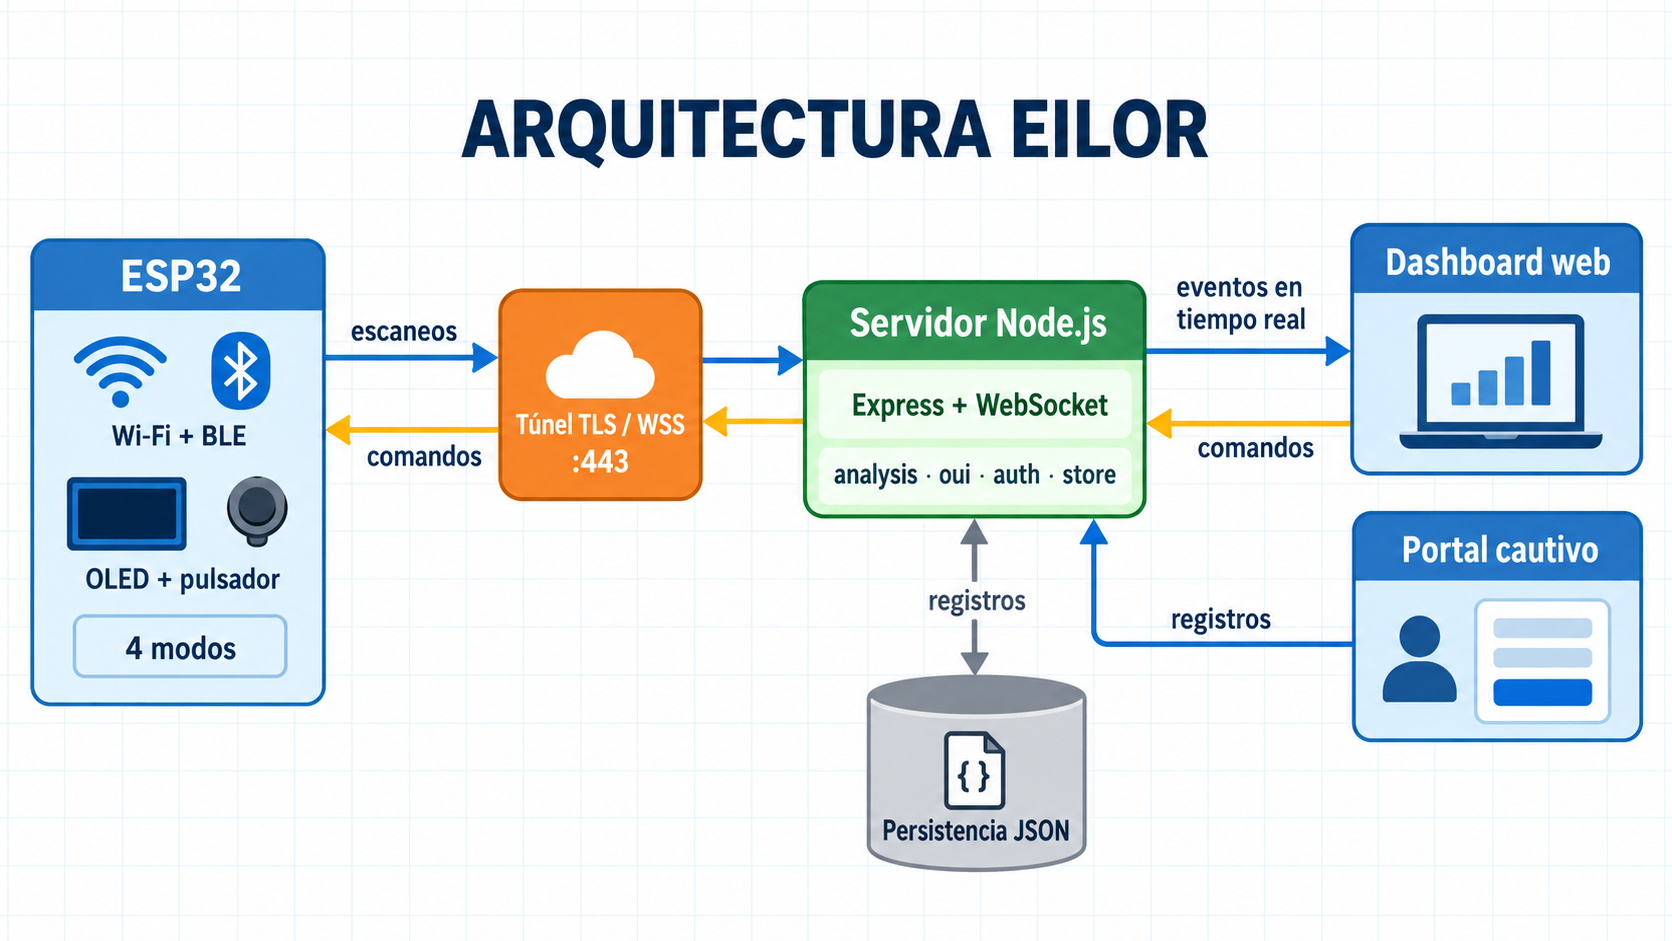
\includegraphics[width=0.98\linewidth]{figuras/arquitectura-eilor}}
\caption{Arquitectura general de EILOR: dispositivo, túnel, servidor modular, persistencia y clientes. La imagen resume el flujo; los contratos de mensajes se especifican en las tablas y diagramas de secuencia del capítulo.}
\label{fig:arquitectura}
\end{figure}

\section{Descripción de las capas}
\subsection{Capa de dispositivo (ESP32)}
El firmware implementa cuatro modos operativos conmutables por un pulsador físico o por comando remoto: (0)~análisis de espectro Wi\nobreakdash-Fi, (1)~radar de proximidad BLE, (2)~punto de acceso SoftAP con portal cautivo y (3)~telemetría/reposo. Una pantalla OLED SSD1306 muestra el estado local, y el dispositivo mantiene una conexión WebSocket persistente con el servidor para transmitir escaneos y recibir comandos.

\subsection{Capa de servidor (Node.js)}
El servidor centraliza la lógica de negocio en cuatro módulos desacoplados dentro de \code{lib/}: \code{analysis} (puntaje de interferencia y detección de gemelos maliciosos), \code{oui} (identificación de fabricante y MAC aleatorizadas), \code{store} (persistencia y series temporales) y \code{auth} (autenticación por token). Sobre ellos, \code{server.js} expone un servidor WebSocket y una API REST de catorce \emph{endpoints}.

\subsection{Capa de clientes}
Dos tipos de clientes consumen el sistema: el \emph{dashboard} web, que recibe actualizaciones en vivo por WebSocket y visualiza el espectro, el radar, la tabla de dispositivos y los registros; y los \emph{invitados}, que al conectarse al SoftAP son redirigidos por el portal cautivo a un formulario de registro.

\section{Selección de tecnologías}
La Tabla~\ref{tab:stack} justifica la pila tecnológica seleccionada.

\begin{table}[H]
\centering
\caption{Pila tecnológica y justificación}
\label{tab:stack}
\footnotesize
\begin{tabularx}{\linewidth}{@{}l l X@{}}
\toprule
\textbf{Capa} & \textbf{Tecnología} & \textbf{Justificación} \\
\midrule
Hardware & ESP32 & Radios Wi-Fi + BLE integradas, bajo costo, pila TCP/IP \parencite{espressif2023} \\
Pantalla & OLED SSD1306 & Bajo consumo, I\textsuperscript{2}C, suficiente para telemetría local \\
Firmware & C++ / Arduino & Ecosistema maduro de librerías (WebSockets, BLE, DNSServer) \\
Servidor & Node.js + Express & E/S no bloqueante idónea para tiempo real \parencite{nodejs2024} \\
Tiempo real & WebSocket (\code{ws}) & Canal bidireccional persistente de baja latencia \parencite{rfc6455} \\
Persistencia & Archivos JSON & Sin dependencias nativas; portable y auditable \\
Portal cautivo & DNSServer + WebServer & Redirección DNS y formulario embebido \parencite{rfc1035} \\
Frontend & HTML/CSS/JS & Sin framework; ligero y transparente \\
Despliegue & PM2 & Gestión de procesos, reinicio y persistencia de arranque \\
\bottomrule
\end{tabularx}
\end{table}

\section{Especificaciones técnicas iniciales}
\begin{itemize}[leftmargin=1.4em]
  \item \textbf{Banda:} 2.4~GHz; canales Wi-Fi 1--13; canales BLE de advertising 37, 38 y 39.
  \item \textbf{Frecuencia de escaneo:} ciclo de $\sim$3~s por modo activo.
  \item \textbf{Telemetría:} \emph{heartbeat} cada 3~s; \emph{watchdog} de desconexión a los 15~s.
  \item \textbf{Series temporales:} una muestra por minuto, retención de 720 muestras ($\sim$12~h).
  \item \textbf{Persistencia:} \emph{snapshot} de dispositivos cada 30~s y volcado en apagado ordenado.
  \item \textbf{Seguridad:} token de sesión (TTL 24~h) para control; token de dispositivo opcional para ingesta.
\end{itemize}
